\subsection{Class diagram}
	The following graphic is the class diagram that we will use for the specification and the implementation.

	%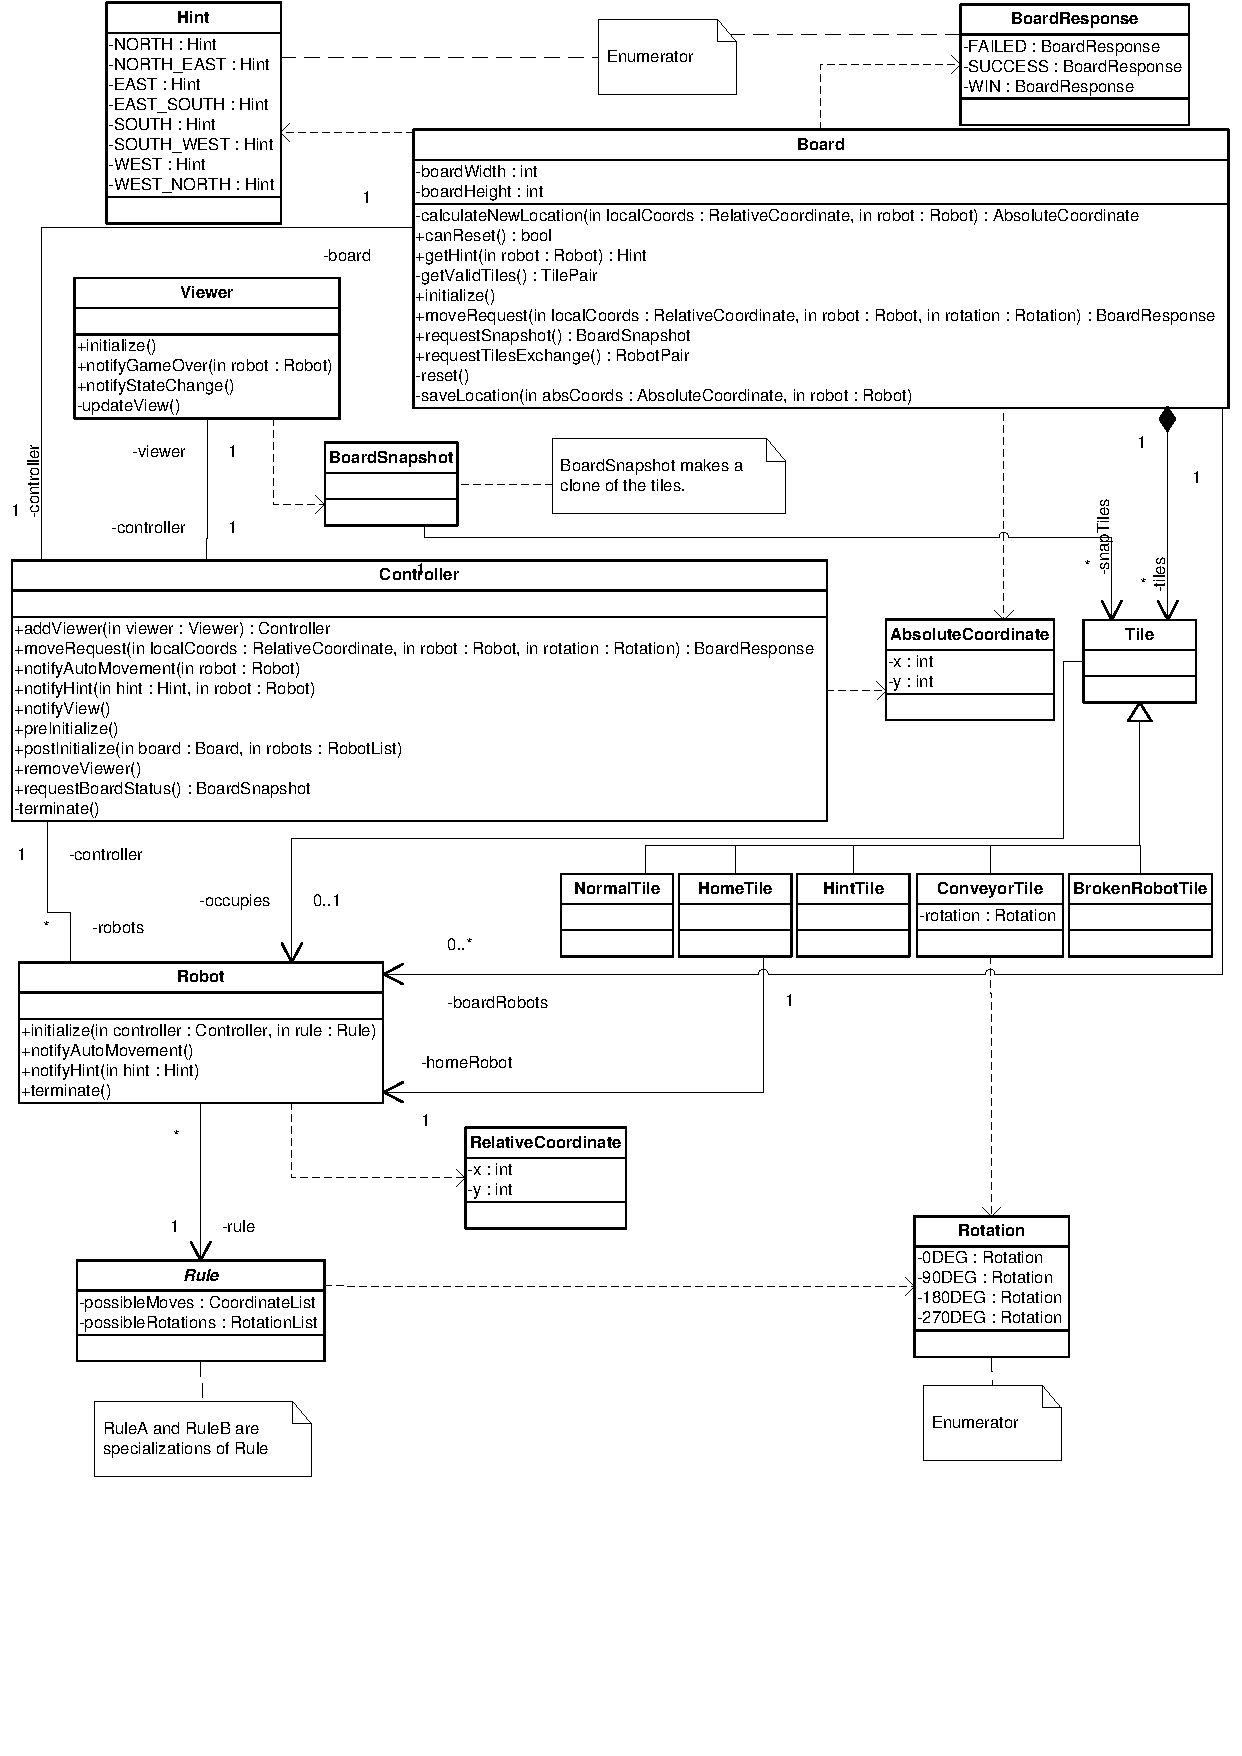
\includegraphics[width=\linewidth]{classdiagram.pdf}
	\let\l=\relax
\let\<=\relax
\let\>=\relax
\digraph[scale=.5]{classdiagram}{
margin=0
fontsize=8
fontname=Helvetica
compound=true
splines=ortho
node [fontsize=8, fontname=Helvetica, shape=record]
edge [fontsize=8, fontname=Helvetica, arrowhead=open, labeldistance=2]
Board [label="{Board|- width : int\l- height : int\l|+ canReset() : bool\l+ initialize()\l+ moveRequest(loc : RelativeCoord, r : Robot, rot : Rotation) : BoardResponse\l+ requestSnapshot() : BoardSnapshot\l+ requestTilesExchange() : bool\l- getHint(r : Robot) : Hint\l- calculateNewLocation(loc : RelativeCoord, r : Robot) :
AbsoluteCoord\l- getValidTiles() : TilePair\l- reset()\l- saveLocation(loc : AbsoluteCoord, r : Robot)\l}"]
Hint [label="{[Hint]| NORTH\l NORTH_EAST\l EAST\l SOUTH_EAST\l SOUTH\l SOUTH_WEST\l WEST\l NORTH_WEST\l}"]
BoardResponse [label="{[BoardResponse]| FAILED\l SUCCESS\l WIN\l}"]
Viewer [label="{Viewer||+ initialize()\l+ notifyGameOver(r : Robot)\l+ notifyStateChange()\l- updateView()\l}"]
BoardSnapshot [label="{BoardSnapshot||}"]
Controller [label="{Controller||+ addViewer(v : Viewer) : Controller\l+ moveRequest(loc : RelativeCoord, r : Robot, rot : Rotation) : BoardResponse\l+ notifyAutoMovement(r : Robot)\l+ notifyHint(h : Hint, r : Robot)\l+ notifyView()\l+ preInitialize()\l+ postInitialize(b : Board, rs : RobotList)\l+ removeViewer()\l+ requestBoardSnapshot() : BoardSnapshot\l- terminate()\l}"]
AbsoluteCoord [label="{AbsoluteCoord|+ x : int\l+ y : int\l|}"]
Tile [label="{Tile||}"]
/**/
subgraph cluster_Tiles {
NormalTile [label="{NormalTile||}"]
HomeTile [label="{HomeTile||}"]
HintTile [label="{HintTile||}"]
ConveyorTile [label="{ConveyorTile|- rot : Rotation|}"]
BrokenRobotTile [label="{BrokenRobotTile||}"]
}
/**/
Robot [label="{Robot||+ initialize(c : Controller, r : Rule)\l+ notifyAutoMovement()\l+ notifyHint(h : Hint)\l+ terminate()\l}"]
RelativeCoord [label="{RelativeCoord|+ x : int\l+ y : int\l|}"]
Rule [label="{\<\<Rule\>\>|- possibleMoves : RelativeCoordList\l- possibleRotations : RotataionList\l|}"]
Rotation [label="{[Rotation]| 0DEG\l 90DEG\l 180DEG\l 270DEG\l}"]
/**/
Board->Controller [taillabel=1, headlabel="0..*"]
Board->Tile [arrowtail=diamond,dir=both, taillabel=1,headlabel="*"]
Board->Robot [taillabel=1, headlabel="0..*"]
/**/
Controller->Viewer [taillabel=1, headlabel=1, arrowhead=none]
Controller->Robot [taillabel=1, headlabel="*", arrowhead=none]
/**/
Tile->Robot [taillabel=1, headlabel="              0..1 - occupier"]
/**/
HomeTile->Robot [taillabel=1, headlabel="              1 - homeRobot"]
/**/
Robot->Rule [taillabel="*", headlabel=1]
/**/
BoardSnapshot->Tile [taillabel=1, headlabel="*"]
/**/
NormalTile->Tile [ltail=cluster_Tiles,arrowhead=empty]
/**/
Board->Hint [style=dashed]
Board->BoardResponse [style=dashed]
Board->AbsoluteCoord [style=dashed]
Viewer->BoardSnapshot [style=dashed]
Controller->AbsoluteCoord [style=dashed]
Robot->RelativeCoord [style=dashed]
Rule->Rotation [style=dashed]
ConveyorTile->Rotation [style=dashed]
} 

\subsection{Class description}
	\begin{description}
		\item[Board] The class for the board as it was given in the informal specification.
		\item[Controller] The main controller as it was given in the informal specification.
		\item[Robot] This is used for both Robot A and Robot B in the informal sepcification.
		\item[Viewer] This is the viewer as it was given in the informal specification.
		\item[Tile] This class is used to model the tiles that the Board consists of.
		\item[NormalTile] This class is a specialization of the Tile class for a normal tile.
		\item[HomeTile] This class is a specialization of the Tile class for a home tile.
		\item[HintTile] This class is a specialization of the Tile class for a hint tile.
		\item[ConveyorTile] This class is specialization of the Tile class for a conveyor tile.
		\item[BrokenRobotTile] This class is a specialization of the Tile class for a broken robot tile.
		\item[Rule] This class is used to model the behaviour of Robot A and B in the Robot class. Any class that defines a rule inherits from this class.
		\item[Rotation] This is an enumeration class that is used to model the rotations of Robot.
		\item[RelativeCoordinate] This is a data class that contains the x and y coordinate of a relative coordinate.
		\item[AbsoluteCoordinate] This is a data class that contains the x and y coordinate of an absolute coordinate.
		\item[Hint] This in an enumeration class that contains all possible hints that a Robot can receive from a hint tile.
		\item[BoardSnapshot] This is a data class that contains a snapshot of the board, i.e. a copy of all the tiles in the board.
		\item[BoardResponse] This in an enumerator that contains all the possible responses that the board can give the controller when it makes a move request.
	\end{description}
